177. \begin{figure}[ht!]
\center{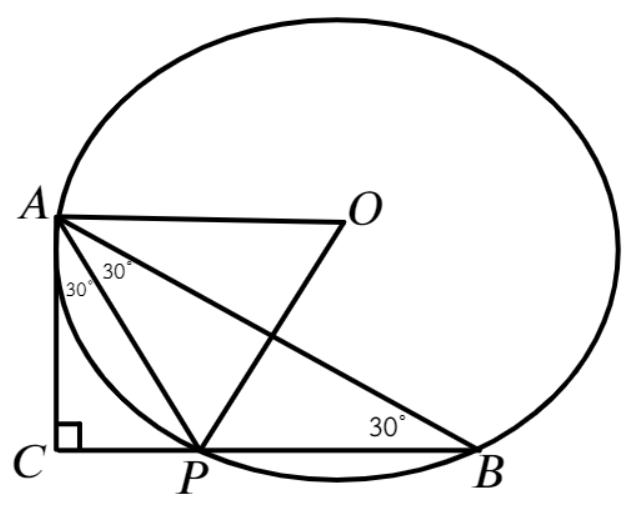
\includegraphics[scale=0.35]{g8-178.png}}
\end{figure}\\
а) Посчитаем углы: $\angle B=90^\circ-60^\circ=30^\circ,\ \angle CAP=\angle BAP=60^\circ:2=30^\circ.$ Тогда треугольник $APB$ является равнобедренным и $AP=PB=4,$ а в прямоугольном треугольнике $ACP$ катет $CP$ лежит напротив угла в $30^\circ,$ значит $CP=AP:2=2.$ По теореме Пифагора $AC=\sqrt{16-4}=2\sqrt{3},$ поэтому $S_{\Delta ABC}=\cfrac{2\sqrt{3}(2+4)}{2}=6\sqrt{3}.$\\
б) $S_{\Delta ABP}=S_{\Delta ABC}-S_{\Delta ACP}=6\sqrt{3}-\cfrac{2\sqrt{3}\cdot2}{2}=4\sqrt{3}.$\\
в) Угол $ABP$ опирается на дугу $AP,$ значит $\smile AP=2\angle ABP=60^\circ.$ Угол $AOP$ является центральным, значит $\angle AOP=60^\circ.$ В треугольнике $AOP$ стороны $AO$ и $OP$ равны радиусу окружности, значит он равнобедренный, а раз угол при его вершине равен $60^\circ,$ то и равносторонний. Поэтому $R=AP=4.$\\
